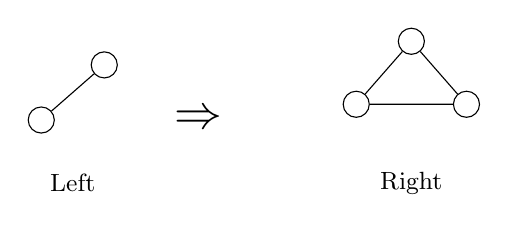
\begin{tikzpicture}[
    small/.style={circle, draw=black, minimum size=6pt},
    arrow/.style={->, thick}
]

\node[small] (L1) at (0,0){};
\node[small] (L2) at (0.8,0.7){};
\draw (L1)--(L2);

\node at (0.4,-0.8) {\small Left};

\node at (2,0) {\LARGE $\Rightarrow$};

\node[small] (R1) at (4,0.2){};
\node[small] (R2) at (4.7,1.0){};
\node[small] (R3) at (5.4,0.2){};

\draw (R1)--(R2)--(R3)--(R1);

\node at (4.7,-0.8) {\small Right};

\end{tikzpicture}